\chapter{Måling af THD i indgangsvælger}
\label{maalejournal_indgangsvaelger_2}

Denne målerapport dokumenterer målinger foretaget på projektets indgangsvaelger, opbygget som beskrevet i kapitel \ref{indgangsvaelger}. Målingen er foretaget på Fredrik Bajers Vej 7 i lokale B1-104 på Aalborg Universitet den 15. december 2010 af gruppe 311.

\subsection*{Formål}
Målingens formål er at måle:
\begin{itemize}
\item THD ved benyttelse af anden operationsforstærker
\item Indvirkningen af transistorerne på THD
\end{itemize}

\subsection*{Testobjekt}
Der vil i denne målerapport blive udført tests af indgangsvælgeren, som vist på figur \ref{maalerap_diagram_simulering}. Testene vil tage udgangspunkt i én indgang; mikrofonindgangen. Dette skyldes at indgangene menes at være så ens, at de vil give samme output som fundet i Appendiks \ref{maalejournal_indgangsvaelger}. Der vil i stedet for en LM324 blive benyttet en OPA27\kilde{OPA27.pdf}.

Til frekvensmåling sendes signalet ind på en tændt indgang, medmindre andet er markeret. Indgangen der ikke benyttes vil så være slukket.
\begin{figure}[h]
\centering
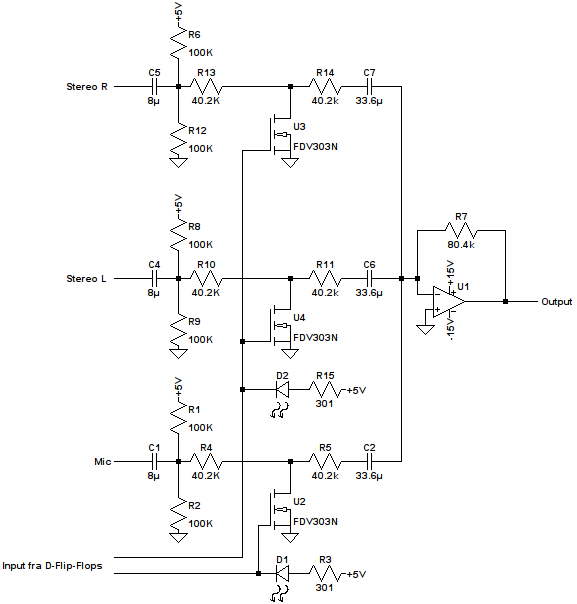
\includegraphics[scale=0.8]{maalerapporter/indgangsvaelger/indgangvaelger_ltspice_diagram.png}
\caption{Diagram over kredsløbet der testes.}
\label{maalerap_diagram_simulering}
\end{figure}

\subsection*{Måleopstilling}
Måleopstillingen er vist på figur \ref{fig:indgangthd:maaleop-thd}.

\begin{figure}[h]
\centering
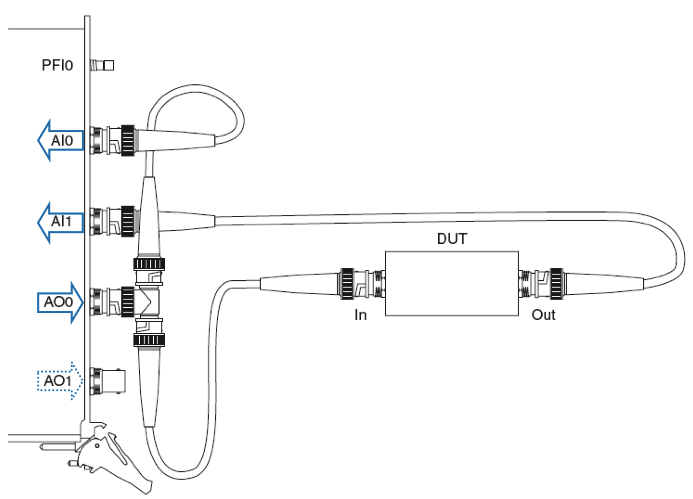
\includegraphics[scale=0.4]{maalerapporter/indgangsvaelger/maaleopstilling-thd-forforstaerker.png}
\caption{Måleopstilling for forstærkning-, frekvensgang- og forvrængningsmåling \cite{maaling-mm5}}
\label{fig:indgangthd:maaleop-thd}
\end{figure}

\subsection*{Anvendt udstyr}
\fixme{clearpage?}
\begin{table}[h]
\centering
\begin{tabular}{l|c|l}
\hline\hline
Instrument & AAU-nr. & Fabrikant, type m.v. \\
\hline\hline
Spændingsforsyning & 39897 & HAMEG HM7042 \\[4pt]
Spændingsforsyning & 33901 & HAMEG HM7042 \\[4pt]
Multimeter & 08518 & Fluke and Philips FLUKE 37 \\[4pt]
Audioanalysator & 76986 & National Instruments NI-PCI-4461 \\
\hline\hline
\end{tabular}
\label{tab:indgang:maaleudstyr_forforstaerker}
\end{table}

\subsection*{Måleprocedure}
\begin{enumerate}
\item En spændingsforsyning indstilles til $\pm$15 V (indstilles med multimeteret) og tilsluttes.
\item En spændingsforsyning indstilles til 5 V (indstilles med multimeteret) og tilsluttes.
\item Testobjektet tilsluttes som på figur \ref{fig:indgangthd:maaleop-thd}
\item Kanalen der måles på, indstilles ved hjælp af trykknappen.
\item Programmet $"$Swept Sine - Linear Response and Harmonic Distortion (DAQmx)$"$ startes
\item $"$Start frequency$"$ under Source settings sættes til 20 Hz
\item $"$Stop frequency$"$ under Source settings sættes til 20 kHz
\item $"$Amplitude$"$ under Source settings sættes til 2 V
\item $"$THD units$"$ sættes til \%
\item $"$AI Range$"$ for Stimulus channel sættes til $\pm$ 0,316 V\fixme{Check}
\item $"$AI Range$"$ for Respons channel sættes til $\pm$ 3,16 V\fixme{dem her}
\item $"$Sampling frequency$"$ sættes til 204,8 kHz
\end{enumerate}

Den første test foretages normalt, som vist på opstillingen. Ved testen uden transistorer fjernes transistorerne.	

\subsection*{Resultater}

THD blev målt for de forskellige opsætninger. Resultaterne vises i figur \ref{fig:apind:200mvm} til figur \ref{fig:apind:2vu}. Resten af resultaterne kan findes på CD'en\fixme{henvisning}. Værdier angivet i V og mV er amplitudespændinger.

\begin{figure}[h]
\centering
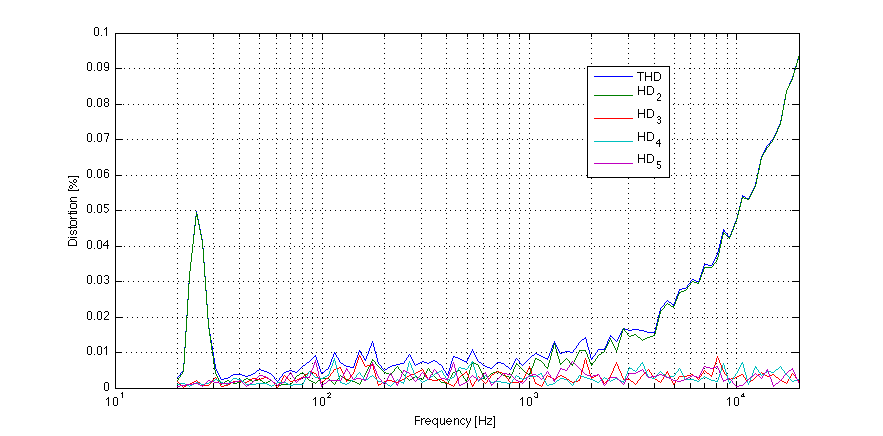
\includegraphics[width=\textwidth]{maalerapporter/indgangsvaelger/maalinger/opa/mic-200mv-opa-muxudgang-thd.png}
\caption{THD ved 200 mV med transistorer}
\label{fig:apind:200mvm}
\end{figure}

\begin{figure}[h]
\centering
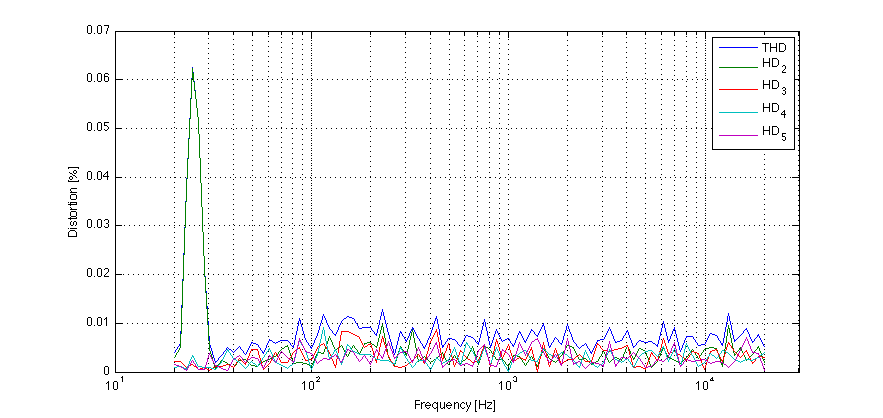
\includegraphics[width=\textwidth]{maalerapporter/indgangsvaelger/maalinger/opa/mic-200mv-opa-muxudgang-uden-transistor thd.png}
\caption{THD ved 200 mV uden transistorer}
\label{fig:apind:200mvu}
\end{figure}

\begin{figure}[h]
\centering
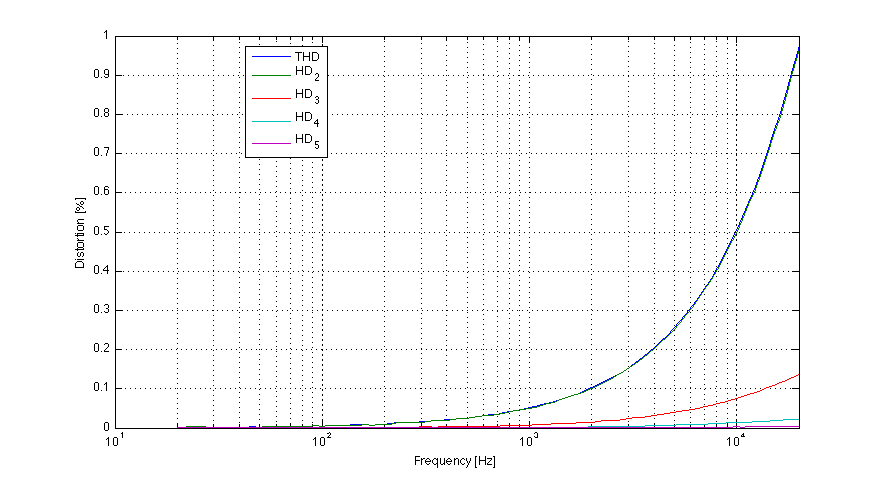
\includegraphics[width=\textwidth]{maalerapporter/indgangsvaelger/maalinger/opa/mic-2v-opa-muxudgang-thd.png}
\caption{THD ved 2 V med transistorer}
\label{fig:apind:2vm}
\end{figure}

\begin{figure}[h]
\centering
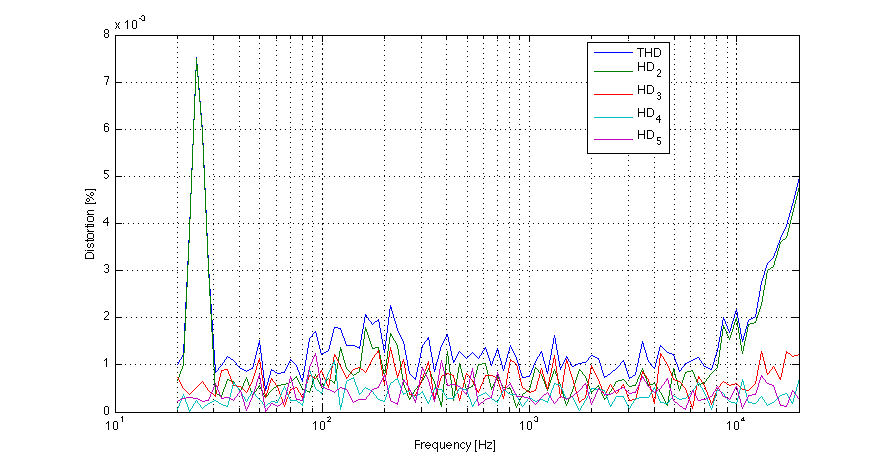
\includegraphics[width=\textwidth]{maalerapporter/indgangsvaelger/maalinger/opa/mic-2v-opa-muxudgang-uden-transistor-thd.png}
\caption{THD ved 2 V uden transistorer}
\label{fig:apind:2vu}
\end{figure}

\clearpage
\subsection*{Måleusikkerheder}
\begin{itemize}
\item Komponent tolerancer
\item Påvirkning fra måleinstrument
\item Måleinstrument unøjagtighed
\item Støj, 50 Hz brum
\item Anden indstråling
\end{itemize}